\chapter{Theoretische Grundlagen}

\section{Klangsynthese}
\label{sec:org6f295e3}
Das Wort \textbf{Synthese} bedeutet in etwa zusammensetzen oder zusammenfügen \cite{duden:synthese}, beschreibt also das Erschaffen von etwas Neuem durch die Vereinigung von kleineren Teilen. Klangsynthese bedeutet also, aus grundlegenden Klangwellen komplexere Klänge zu erzeugen.

Ein \textbf{Synthesizer} ist ein (meist elektronisches) Instrument, welches zur Klangsynthese fähig ist. Während die meisten herkömmlichen analogen Instrumente nur eine oder wenige unterschiedliche Klangfarben erzeugen können, ist eine der Kernaufgaben eines Synthesizers das Erzeugen von Klängen mit beliebig änderbarer Klangfarbe. Zwar können Synthesizer auch herkömmliche Instrumente imitieren, vor allem sind sie jedoch das Mittel der Wahl, wenn unnatürliche und untypische Klangfarben erzeugt werden sollen oder wenn sich die Klangfarbe eines Tones ändern soll, während er gespielt wird.

\subsection{Klangwellen}
\label{sec:org4f3ced6}
Klangwellen sind die Grundbausteine der Klangsynthese. Sie können in verschiedenen Medien vorkommen, beispielsweise als Spannungsänderungen, welche wir mit Elektronik manipulieren können oder als Schallwellen in der Luft. Weitere Formen von Klangwellen sind die Schwingungen einer Gitarrensaite oder einer Lautsprechermembran, welche ihre Umgebungsluft in Schwingung versetzen und dadurch Schallwellen erzeugen oder auch Elektromagnetische Wellen beim Funk.

\subsubsection{Frequenz \label{frequenz}}
\label{sec:org7da1e05}
Die Tonhöhe einer Klangwelle hängt von ihrer \textbf{Frequenz} ab, also von der Geschwindigkeit, in welcher sie schwingt. Dabei nimmt das menschliche Gehirn Töne auf eine logarithmische Art und Weise wahr, um eine große Bandbreite an Tonhöhen differenzieren zu können. Aus diesem Grund entspricht ein Ton mit der doppelten Frequenz dem selben Ton eine Oktave höher. Die Einheit für Frequenzen ist \si{\hertz} und entspricht \(\frac{1}{\si{\second}}\), drückt also aus, wie oft eine Welle in einer Sekunde schwingt.

\subsubsection{Amplitude \label{amplitude}}
\label{sec:org3ac76ae}
Die Lautstärke einer Klangwelle korrespondiert mit ihrer \textbf{Amplitude} und wird in der Regel in Bel bzw. üblicherweise ein Zehntel Bel, also Dezibel (\si{\dB}) angegeben. Bel ist eine relative Einheit, welche genutzt wird, um das Energieverhältnis zweier Signale zu vergleichen.

Bei Schallwellen wird üblicherweise die Amplitude mit der kleinsten hörbaren Luftdruckänderung (\SI{20}{\micro\pascal}) verglichen. Dadurch wird aus der relativen Einheit (dezi)Bel die absolute Einheit \si{\dB}\textsubscript{SPL} (SPL steht für Sound Pressure Level), welche umgangssprachlich oft fälschlicherweise als \si{\dB} bezeichnet wird.

Da das menschliche Gehör Lautstärke auf eine logarithmische Art und Weise wahrnimmt, ist auch die Bel-Skala eine logarithmische. So bedeutet eine Steigerung der Lautstärke um 20 \si{\dB} eine verzehnfachung der Amplitude, also des Energieniveaus der Welle (siehe Abbildung \ref{fig:org94691f1}).

\begin{figure}[htbp]
\centering
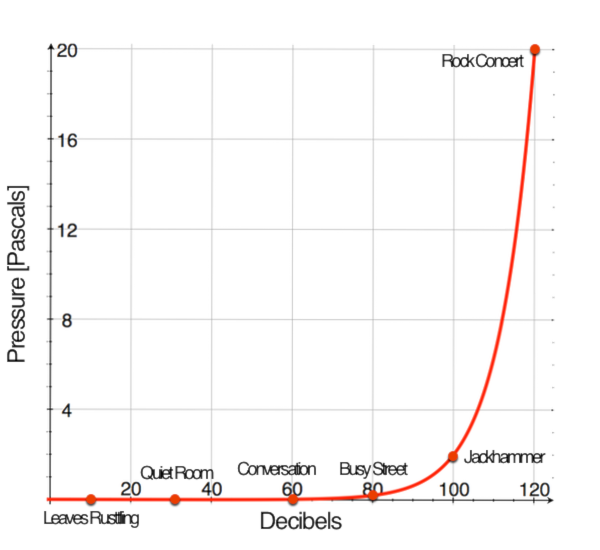
\includegraphics[height=200px]{/home/felixp/Documents/diplomarbeit/dokumentation/figures/decibel_scale.png}
\caption{\label{fig:org94691f1}Dezibelskala mit häufigen Lautstärken als Referenzpunkte und zugehörigen Luftdrucksänderungen in Pascal \cite{at:decibels}}
\end{figure}

Auch nimmt der Mensch gewisse Frequenzen lauter wahr als andere, Frequenzen außerhalb des hörbaren Bereichs können beispielsweise gar nicht wahrgenommen werden. Deshalb kann eine Gewichtungsfunktion, genannt A-weighting, auf den Lautstärkewert angewendet werden. Dieser \textbf{bewertete Schalldruckpegel} wird als \si{\dB}\textsubscript{A} bezeichnet und dient zum Ausdrücken der gefühlten Lautstärke (siehe Abbildung \ref{fig:org35b07cb}).

\begin{figure}[htbp]
\centering
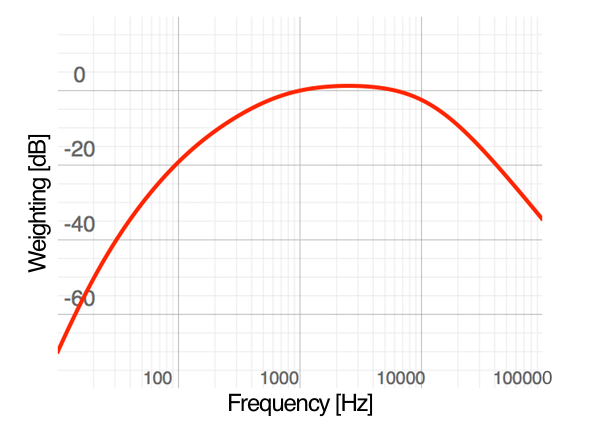
\includegraphics[width=250px]{/home/felixp/Documents/diplomarbeit/dokumentation/figures/a_weighting.png}
\caption{\label{fig:org35b07cb}Gewichtungsfunktion; Hörbare Frequenzen auf der Abszisse, Hörbarkeit durch das menschliche Gehör auf der Ordinate \cite{at:decibels}}
\end{figure}

\subsubsection{Wellenform}
\label{sec:orgc5d98cc}
Klangwellen können verschiedene Formen besitzen, die grundlegende Form ist dabei eine \textbf{Sinuswelle}. Das menschliche Ohr empfindet eine sinusförmige Schallwelle als "`rein"', da sie eine einzelne Frequenz ohne \textbf{Obertöne} repräsentiert. Weitere einfache Formen sind Rechteckwellen, Sägezahnwellen und Dreieckwellen. Im Gegensatz zum Sinus besitzen diese Wellenformen viele Obertöne, welche dem Klang Farbe verleihen. Teilt die Frequenz eines solchen Obertons die Frequenz des Grundtones ganzzahlig, wird er als \textbf{harmonisch}, also wohlklingend empfunden \cite{obertoene}.

Da Wellenformen wie Dreieck-, Rechteck- oder Sägezahnwellen viele Obertöne besitzen \cite{swphonetics:waveforms}, eignen sie sich besonders gut als Grundtöne für die subtraktive Klangsynthese. 

\subsection{Klangerzeugung}
\label{sec:org64c5e90}
Die für die Klangsynthese benötigten grundlegenden Klangwellen können aus verschiedensten Quellen stammen. Die häufigste davon ist wohl ein \textbf{Oszillator}, welcher durchgehende Klangwellen mit einer einfachen Wellenform, wie zum Beispiel einem Sinus oder einer Rechteckwelle generiert. In Abschnitt \ref{Osci} werden Aufbau und Design eines solchen Oszillators beschrieben.

Des weiteren kann ein breites Spektrum von elektronischen Musikinstrumenten und Klangquellen wie E-Gitarren, Thereminen, Radios und Kassettenspielern die zu modifizierenden Klangwellen für einen Synthesizer bereitstellen.

\subsection{Subtraktive Klangsynthese \label{subKS}}
\label{sec:orged19cbd}
Das Prinzip der subtraktiven Klangsynthese besteht darin, Grundtöne mit vielen Obertönen zu filtern, um Töne mit einer gewünschten Klangfarbe zu erzeugen. Durch einen \textbf{Filter} wird die Amplitude von Teilwellen unter einer bestimmten Frequenz (=> high-pass Filter) oder über einer bestimmten Frequenz (=> low-pass Filter) verringert, wodurch zum Beispiel unangenehme hohe Obertöne gefiltert werden können.

Nach einen solchen Filter wird oft ein \ac{VCA} (siehe Abschnitt \ref{VCA}) geschalten, welcher die Amplitude des Eingangssignals proportional zur angelegten \acl{CV} (siehe Abschnitt \ref{CV}) skaliert. Diese \acl{CV} kann beispielsweise durch einen \ac{LFO} (siehe Abschnitt \ref{LFO}) oder Hüllkurvengenerator (siehe Abschnitt \ref{AR}) bereitgestellt werden. Durch einen \ac{VCA} kann einem durchgehend gleich lauten Klang Dynamik und Rhythmus verliehen werden, indem seine Lautstärke mit dem Verlauf der Zeit geändert wird.

Die meisten analogen Synthesizer basieren auf subtraktiver Klangsynthese. Üblicherweise wird dabei ein Grundton, meist aus einem Oszillator, über einen \ac{VCA} geschalten, welcher durch einen Hüllkurvengenerator angesteuert wird. Dieser Hüllkurvengenerator wird üblicherweise durch einen Sequenzer oder eine Tastatur angesteuert. Eine Abwandlung dieser grundlegenden \textbf{Signalverarbeitungskette} ist in den meisten kommerziell erhältlichen Synthesizersystemen fest verkabelt.

\subsection{Additive Klangsynthese}
\label{sec:org9aa0cf3}
Nach Fourier kann jegliche Art von Wellenform durch eine Serie von Sinuswellen ausgedrückt werden. Das Prinzip der additiven Klangsynthese besteht somit darin, eine Vielzahl von Sinuswellen mit unterschiedlichen Amplituden und Frequenzen zu kombinieren \cite{soundtraining:synthesis} (beispielsweise durch einen Mixer, siehe Abschnitt \ref{Mixer}), um Klänge mit jeder erdenklichen Klangfarbe zu erzeugen. Idealerweise wird jede grundlegende Sinuswelle durch eine separate Hüllkurve moduliert, um einen Klang mit sich laufend verändernder Klangfarbe zu erzeugen \cite{raffaseder}. Da dies mit einer steigenden Anzahl an grundlegenden Sinuswellen eine technische Herausforderung darstellt, sind additive Synthesizer meist digital ausgeführt, ein analoges Beispiel für einen additiven Synthesizer wäre eine \textbf{Hammond-Orgel} \cite{delamar:synthesis}.

\subsection{Vocoder}
\label{sec:org6d1d8f3}
Ein Vocoder basiert auf dem Prinzip, ein Signal (meist eine Stimme) mittels mehrerer Band-Pass Filter in seine Frequenzbestandteile aufzuteilen. Anschließend wird dieses Frequenzspektrum auf der Basis von weißem Rauschen (siehe Abschnitt \ref{Noise}) wieder aufgebaut, um einen als gesprochenes Wort zu erkennenden Klang zu erzeugen. Ein Vocoder arbeitet somit sowohl mit subtraktiver Soundsynthese bei der Analyse des Frequenzspektrums als auch mit additiver Soundsynthese beim Wiederzusammensetzen des analysierten Klangs.

\section{Geschichte}
\label{sec:org71defe3}
Bereits im frühen 20. Jahrhundert wurden elektronische Schaltkreise benutzt, um Klänge zu erzeugen. Damals noch mit Vakuumröhren statt Transistoren hergestellt, stellt das \textbf{Theremin} eines der ältesten heute noch verwendeten elektronischen Musikinstrumente dar \cite{thomann:theremin}. 

Der erste vollwertige elektronische Synthesizer, welcher auch als solcher bezeichnet wurde, war der \textbf{RCA Music Synthesizer}, eine raumhohe Maschine, welche als Gemeinschaftsprojekt zwischen den amerikanischen Universitäten von Princeton und Columbia entstanden war. Statt mit einer Klaviertastatur spielte beziehungsweise programmierte man diesen Synthesizer erst mittels Lochkarten und konnte dann gewisse Aspekte des Klanges dynamisch - also während das Stück spielte - ändern.

Das Konzept eines modularen Synthesizers und damit auch das Konzept der \acl{CV} wurde erstmals von Robert Moog in seiner Arbeit mit dem Titel "`VOLTAGE-CONTROLLED ELECTRONIC MUSIC MODULES"' dokumentiert \cite{moog1964}. Der auf diesen Prinzipien basierende \textbf{Moog Modular Synthesizer} führte viele heute noch aktuelle Standards ein, wie zum Beispiel die Kontrollspannungsarten Trigger und \SI{1}{\volt} pro Oktave, auf welche in Abschnitt \ref{CV} näher eingegangen wird. Spätestens mit dem 1968 erschienenen Album "`Switched-On Bach"' von Wendy Carlos wurde der Synthesizer als vollwertiges Instrument im Mainstream akzeptiert \cite{yamaha:history} \cite{120years:moog}. 

Während die Synthesizer von Moog mit dem Prinzip der subtraktiven Klangsynthese arbeiteten, wurden zur gleichen Zeit - auf der anderen Seite Amerikas - erste Synthesizer mit additiver Klangsynthese hergestellt. Die von \textbf{Donald Buchla} hergestellten Synthesizer boten dem Benutzer beinahe grenzenlose Freiheit über die Farbe der erzeugten Klänge. Dennoch blieb die subtraktive Klangsynthese wohl aufgrund größerer Intuitivität und besserer technischer Umsetzbarkeit das vorherrschende Prinzip \cite{120years:buchla}. 

Obwohl Moog als Vater der modularen Klangsynthese gilt, ist eines der bekanntesten und beliebtesten Produkte der Firma Moog der fix verkabelte \textbf{Minimoog}. Dieser als Live-Instrument gedachte Synthesizer führte ein Lautstärkerad und ein Tonhöhenveränderungsrad ein, mit welchem Töne ähnlich wie beim Saitenziehen bei einer Gitarre verändert werden können \cite{120years:moog}.

Die 1970er und 1980er Jahre waren vor allem von digitalen Synthesizern geprägt. Das von der Firma "`New England Digital"' hergestellte Synclavier I war der erste Synthesizer welcher Frequenzmodulation, eine Form der additiven Klangsynthese anbot. Der von Yamaha hergestellte \textbf{DX7} brachte dieses Konzept in den Mainstream. Die glockenartigen Klänge die charakteristisch für diese Art der Klangsynthese sind, prägten den Großteil der 80er Jahre und sind auch heute noch häufig in Pop und Schlager zu finden \cite{yamaha:history}.

Das Konzept der modularen Synthesizer schien beinahe vergessen, bis im Jahre 1996 Dieter Döpfer das modulare Synthesizersystem \textbf{A-100} entwarf. Die quelloffene Natur dieses Systems ermöglichte es anderen Herstellern wie auch den Firmen Moog, Rohland und Behringer, kompatible Module herzustellen, wodurch ein De-facto-Standard, heute bekannt als Eurorack, entstand. Dieser Standard führte zu einer Renaissance der modularen Synthesizer, heutzutage basieren fast alle modularen Synthesizer auf dem Eurorack-Format.

Die Dokumentation für diesen Synthesizer, den A-100, stellt auf direkte oder indirekte Weise die Grundlage für die meisten Aspekte des in der vorliegenden Arbeit beschriebenen Systems dar.

\section{Das Eurorack-Format}
\label{sec:org39b59ec}

Der 1996 von der Doepfer Musikelektronik GmbH veröffentlichte A-100 Synthesizer benutzte für viele Zwecke bereits etablierte Maße und Werte. Beispielweise werden die durch den Moog Modular Synthesizer popularisierten Kontrollspannungsarten benutzt. Auch die physischen Dimensionen der Module basierten auf einem bereits vorhandenen Standard, dem Eurocard-Standard (IEEE 1101.1). Der Begriff Eurorack stammt wohl vom Namen dieses Standards ab. Bald nach der Veröffentlichung des A-100 wurden kompatible Module von anderen Herstellern veröffentlicht, wodurch das Eurorack-Format zum De-facto-Standard für modulare Synthesizer wurde. Heute gibt es tausende von Eurorack-Modulen, hergestellt von bekannten Firmen wie Moog, Roland, Behringer und auf Eurorack spezialisierten Herstellern wie Make Noise und Intellijel. Des Weiteren gibt es eine lebendige DIY-Szene mit vielen öffentlichen und quelloffenen Designs, Anleitungen, Schematics und vorgefertigten Kits zum Zusammenbauen.

\subsection{\acf{CV} \label{CV}}
\label{sec:org241e9a5}
Essentiell bei Eurorack-Modulen ist, dass viele Parameter nicht nur durch den Benutzer (durch Knöpfe, Potentiometer, etc.), sondern auch durch andere Module mithilfe von sogenannter \acl{CV} ansteuerbar sind. So kann beispielsweise die Frequenz eines Oszillators, der Cutoff eines Filters, Attack- und Releaselänge einer Hüllkurve und ähnliches durch \acl{CV} kontrolliert werden. Diese \acl{CV} kann wiederum aus verschiedensten Modulen wie z.B. einem MIDI Interface, einem \ac{LFO}, einem Hüllkurvengenerator, welcher zum Beispiel \ac{ADSR} beherrscht, oder sogar einem anderen Audiosignal kommen. Dadurch entsteht ein Netzwerk an elektronischen Schaltungen, welche sich gegenseitig beeinflussen und hochschaukeln, was idealerweise zu wohlklingenden, jedoch in jedem Fall interessanten Effekten führt.

Besonders für Eurorack und für modulare Synthesizer im Generellen hat dieses Konzept einen hohen Stellenwert, da bei solchen Systemen Audiosignale und \acl{CV}en nicht fix verkabelt sind, sondern vom Benutzer flexibel mit \SI{3.5}{\milli\meter} mono Klinkensteckern, sogenannten \textbf{Patchkabeln}, geschalten werden können. Der Unterschied zwischen Audiosignalen und \acl{CV} liegt rein im Verwendungszweck, oft können auch Audiosignale als \acl{CV} dienen. Es gibt verschiedene Arten von \acl{CV}en, welche sich ebenfalls primär durch ihren Verwendungszweck unterscheiden:

\subsubsection{Trigger}
\label{sec:org31fb120}
Triggersignale sind steigende Flanken, meist direkt gefolgt von einer fallenden Flanke, zwischen \SI{0}{\volt} und \SI{5}{\volt}. Ihr Zweck ist es, Prozesse, wie etwa das Fortschreiten eines Sequencers, auszulösen.

\subsubsection{Gate}
\label{sec:orgb6b5394}
Ähnlich wie ein Triggersignal ist ein Gate eine steigende Flanke gefolgt von einer fallenden Flanke zwsichen \SI{0}{\volt} und \SI{5}{\volt}. Im Unterschied zum Trigger ist jedoch der zeitliche Abstand zwischen steigender und fallender Flanke oft beträchtlich länger und spielt eine wichtige Rolle. Gate-Signale werden oft verwendet, um den Zustand einer Keyboardtaste zu beschreiben.

\subsubsection{Hüllkurve}
\label{sec:orgb08c536}
Hüllkurven sind \acl{CV}en, welche oberflächlich einem Gate-Signal ähneln, jedoch spielt der genaue Verlauf der Spannung einer Hüllkurve eine wichtige Rolle. Oft werden Hüllkurven zum Ansteuern von \acp{VCA} oder \acp{VCF} benutzt. Eine häufige Art von Hüllkurve ist \ac{ADSR}, welche den Verlauf der Lautstärke eines Tones beim Drücken einer Taste beschreibt \cite{envelopes}.

\begin{enumerate}
\item \textbf{Attack:}
\label{sec:org79dc270}
Der "'Attack"' Wert gibt an, wie lange der Ton nach dem Drücken der Taste braucht, um auf seine maximale Lautstärke anzuschwellen.

\item \textbf{Decay:}
\label{sec:orgeeb14e5}
Nachdem der Ton seine maximale Lautstärke erreicht hat, schwillt er auf eine niedrigere Lautstärke ab. Der Decay-Wert, gibt an, wie lange der Ton benötigt, um diese niedrigere Lautstärke zu erreichen.

\item \textbf{Sustain:}
\label{sec:orgb7671ae}
Im Unterschied zu den anderen Parametern ist der Sustain-Wert eine Amplitude anstatt einer Zeit. Der eingestellte Wert gibt an, auf welche Lautstärke das Signal nach dem Ablaufen der Decay-Zeit abschwillt. Die eingestellte Lautstärke ist konstant, solange die Taste gedrückt bleibt.

\item \textbf{Release:}
\label{sec:org7cb143a}
Nach dem Loslassen der Taste benötigt der Ton eine gewisse Zeit, um vollständig abzuschwellen.  Diese Zeit wird über den Release-Parameter eingestellt.

\begin{figure}[htbp]
\centering
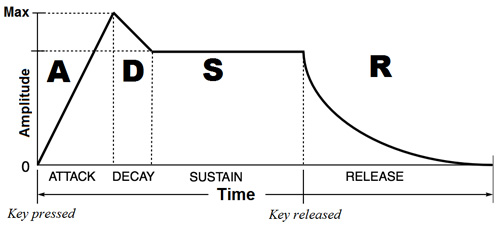
\includegraphics[width=250px]{/home/felixp/Documents/diplomarbeit/dokumentation/figures/ADSR.jpg}
\caption{Der zeitliche Verlauf einer ADSR Hüllkurve; die Amplitudenwerte auf der Ordinate entsprechen bei einem Hüllkurvengenerator den ausgegebenen Kontrollspannungswerten  \cite{envelopes}}
\end{figure}
\end{enumerate}

\subsubsection{Volt per Octave}
\label{sec:org61132ac}
Die meisten \acsp{VCO} folgen der von Moog eingeführten Konvention, dass ihre Frequenz auf eine logarithmische Art und Weise von der \acl{CV} abhängt. Dabei resultiert die Zunahme der \acl{CV} um \SI{1}{\volt} in der Verdoppelung der Frequenz des generierten Signals (1 Oktave).

\subsubsection{Audio}
\label{sec:org3cfa8fa}
Audiosignale sind Spannungen, die meist zwischen \SI{-0.5}{\volt} und \SI{0.5}{\volt} schwingen. Sie können an einen Verstärker oder Lautsprecher angelegt werden, um Schall zu erzeugen oder zur Weiterverarbeitung von einem Modul zum anderen geschickt und sogar als \acl{CV} verwendet werden. 
